\chapter{Prospects on differential \textsl{t}-channel measurements at 13~TeV}
\label{ch:prospects}

\intro{Prospects on extending the presented measurement in Ch.~\ref{ch:diff13} are discussed. \Acrlong{pp} collision data corresponding to 36~\invfb recored with the \gls{cms} experiment in 2016 are utilized for this study. Potential improvements in the training of \acrlongpl{bdt}, the fitting procedure, and in the unfolding are demonstrated. In particular, the measurement of differential cross sections at particle level is envisaged. The presented technical studies of fiducial definitions for $t$-channel single-top-quark events have been published in Ref.~\cite{particleStudies}.}

\todo{update note ref}

\todo{fix all headers of electron plots}

%##############################################
\section{Setup}
%##############################################

The analysis strategy which has been developed in the context of the first measurement of differential cross section of $t$-channel single-top-quark-production (Ch.~\ref{ch:diff13}) is extended as follows. The data statistics is increased by using \gls{pp} collision data recored in 2016 with the \gls{cms} detector at a \acrlong{cm} energy of 13~\TeV corresponding to 36~\invfb. Events containing an isolated muon candidate and two or three jets are selected utilizing mostly the criteria detailed in Sec.~\ref{sec:diff13-selection} with a few exceptions as outlined in the following. Due to the higher instantaneous luminosity in the 2016 data-taking period compared to 2015 which peaked at $15.3~\mathrm{Hz}/\mathrm{nb}$~\cite{lumipublic}, the threshold of the employed single muon trigger has been raised to $24~\GeV$. Consequently, muon candidates with a higher threshold of $\pt>26~\GeV$ are required offline as well. All other muon selection criteria are kept the same. Events containing single electrons and two or three jets are envisaged for a potential update of the differential cross section measurement as well. Data events are recorded with an electron trigger that requires an electron candidate with a transverse momentum of at least $32~\GeV$ within $|\eta|<2.1$ and to fulfill additional tight identification criteria. Electron events for analysis must have a corresponding electron candidate with $\pt>35~\GeV$ within $|\eta|<2.1$. Tight identification criteria have to be fulfilled by the candidate which have been specifically designed to select the most genuine electrons~\cite{CMS-DP-2017-004}.


\gls{cmva}~\cite{CMS-PAS-BTV-15-001}

\todo{add samples and event selection here as well}


\myfigure[p]{\label{fig:pospects-met-wjets} Distributions of the transverse missing energy in the (a)~electron and (b)~muon channel 2j0t control region.}{
\subfloat[]{\adjincludegraphics[height=4.8cm,trim={0 0 {0.16\width} 0},clip]{figures/prospects/plots/2j0t/electron_2j0t_met_qcdnone_nol.pdf}}
\subfloat[]{\adjincludegraphics[height=4.8cm,trim={0 0 {0.\width} 0},clip]{figures/prospects/plots/2j0t/muon_2j0t_met_qcdnone.pdf}}
}

\myfigure[p]{\label{fig:pospects-topmass} Distributions of the reconstructed top quark mass for (left column)~electron and (right column)~muon channel: (top row)~signal region; (bottom row)~\ttbar control region.}{
\subfloat[]{\adjincludegraphics[height=4.8cm,trim={0 0 {0.16\width} 0},clip]{figures/prospects/plots/2j1t/electron_2j1t_top_mass_qcdnone_nol.pdf}}
\subfloat[]{\adjincludegraphics[height=4.8cm,trim={0 0 {0.\width} 0},clip]{figures/prospects/plots/2j1t/muon_2j1t_top_mass_qcdnone.pdf}}\\
\subfloat[]{\adjincludegraphics[height=4.8cm,trim={0 0 {0.16\width} 0},clip]{figures/prospects/plots/3j1t/electron_3j1t_top_mass_qcdnone_nol.pdf}}
\subfloat[]{\adjincludegraphics[height=4.8cm,trim={0 0 {0.\width} 0},clip]{figures/prospects/plots/3j1t/muon_3j1t_top_mass_qcdnone.pdf}}
}






%##############################################
\section{Extended BDT training}
%##############################################

The following observables have been chosen as input to the \gls{bdt} training:

\begin{itemize}
\item the invariant mass of the reconstructed top quark candidate;
\item the missing transverse energy, \met;
\item the transverse momentum of the dijet system, $(\vec{p}_\mathrm{b}+\vec{p}_{\jprime})_\mathrm{T}$;
\item the event shape C as introduced in Sec.~\ref{sec:diff13-bdt};
\item the $\Delta R$ distance between the two jets;
\item the $\Delta R$ distance between the b-tagged jet and the lepton;
\item the invariant mass of the \acrlong{cm} system; $\sqrt{\hat{s}}=|p_\mathrm{top}+p_{\jprime}|$;
\item the W~boson helicity angle, defined between the top quark and lepton momentum in the W~boson rest frame (see Sec.~\ref{sec:theory-top-quark-decay} for details), $\cos\theta_\mathrm{W}^\star$;
\end{itemize}

In particular, the 

\myfigure[p]{\label{fig:prospects-cosWhel} Distributions of the W~boson helicity angle in 2j1t (a)~electron and (b)~muon channel.}{
\subfloat[]{\adjincludegraphics[height=4.8cm,trim={0 0 {0.16\width} 0},clip]{figures/prospects/plots/2j1t/electron_2j1t_cosTheta_wH_qcdnone_nol.pdf}}
\subfloat[]{\adjincludegraphics[height=4.8cm,trim={0 0 {0.\width} 0},clip]{figures/prospects/plots/2j1t/muon_2j1t_cosTheta_wH_qcdnone.pdf}}
}



\myfigure[p]{\label{fig:prospects-bdt-tt} Distributions of the \bdttt discriminant, trained to separate \ttbar from \wjets events, in 2j1t (a)~electron and (b)~muon channel.}{
\subfloat[]{\adjincludegraphics[height=4.8cm,trim={0 0 {0.16\width} 0},clip]{figures/prospects/plots/2j1t/electron_2j1t_bdt_ttw_boost04_CR_nol.pdf}}
\subfloat[]{\adjincludegraphics[height=4.8cm,trim={0 0 {0.\width} 0},clip]{figures/prospects/plots/2j1t/electron_2j1t_bdt_ttw_boost04_CR.pdf}}
}

\myfigure[p]{\label{fig:prospects-bdt-tch} Distributions of the \bdttch discriminant, trained to separate signal from \ttbar and \wjets events, in 2j1t (a)~electron and (b)~muon channel.}{
\subfloat[]{\adjincludegraphics[height=4.8cm,trim={0 0 {0.16\width} 0},clip]{figures/prospects/plots/2j1t/electron_2j1t_bdt_tch_boost04_qcdnone_blind_nol.pdf}}
\subfloat[]{\adjincludegraphics[height=4.8cm,trim={0 0 {0.\width} 0},clip]{figures/prospects/plots/2j1t/muon_2j1t_bdt_tch_boost04_qcdnone_blind.pdf}}
}

%##############################################
\section{Fiducial studies}
%##############################################
\label{sec:prospects-fiducial-studies}



Figures~\ref{fig:prospects-particle-level-muonpt} and~\ref{fig:prospects-particle-level-muoneta} show a comparison of the muon $\pt$ and pseudorapidity at reconstruction, particle, and parton level after selecting events with one muon at each level respectively. The top panels demonstrate a high overlap of the events selected at reconstruction level with the ones at particle and parton level. The acceptance rises with the muon momentum from about 40\% to 90\% due to the relative isolation requirement for reconstructed muons. The number of jets is presented in Fig.~\ref{fig:prospects-particle-level-njet}. Due to the jet energy scale correction, 


dressed leptons (cone algorithms associates photons to leptons but does not cluster close leptons), tau decays, jet clustering (no neutrinos/leptons), b-tagging,




particle level overlap: tightMu: >99\%, 2jets: 80\%, 2j1t: 70\%


\myfigure[p]{\label{fig:prospects-particle-level}Comparison of expected event densities for $1~\invfb$ at $13~\TeV$ after applying the event selection at reconstruction, particle, and parton level respectively:  (a)~muon $\pt$, (b)~muon rapidity, and (c)~number of jets after requiring one isolated and tight muon; (d)~number of b-tagged jets, (e)~$\pt$ and (f)~pseudorapidity of the spectator jet after requiring one isolated, tight muon and two jets where in (e,f) one jet is additionally required to be b-tagged at reconstruction level. Top panels show the common events selected at reconstruction level while the bottom panels display the acceptance.}{
\subfloat[\label{fig:prospects-particle-level-muonpt}]{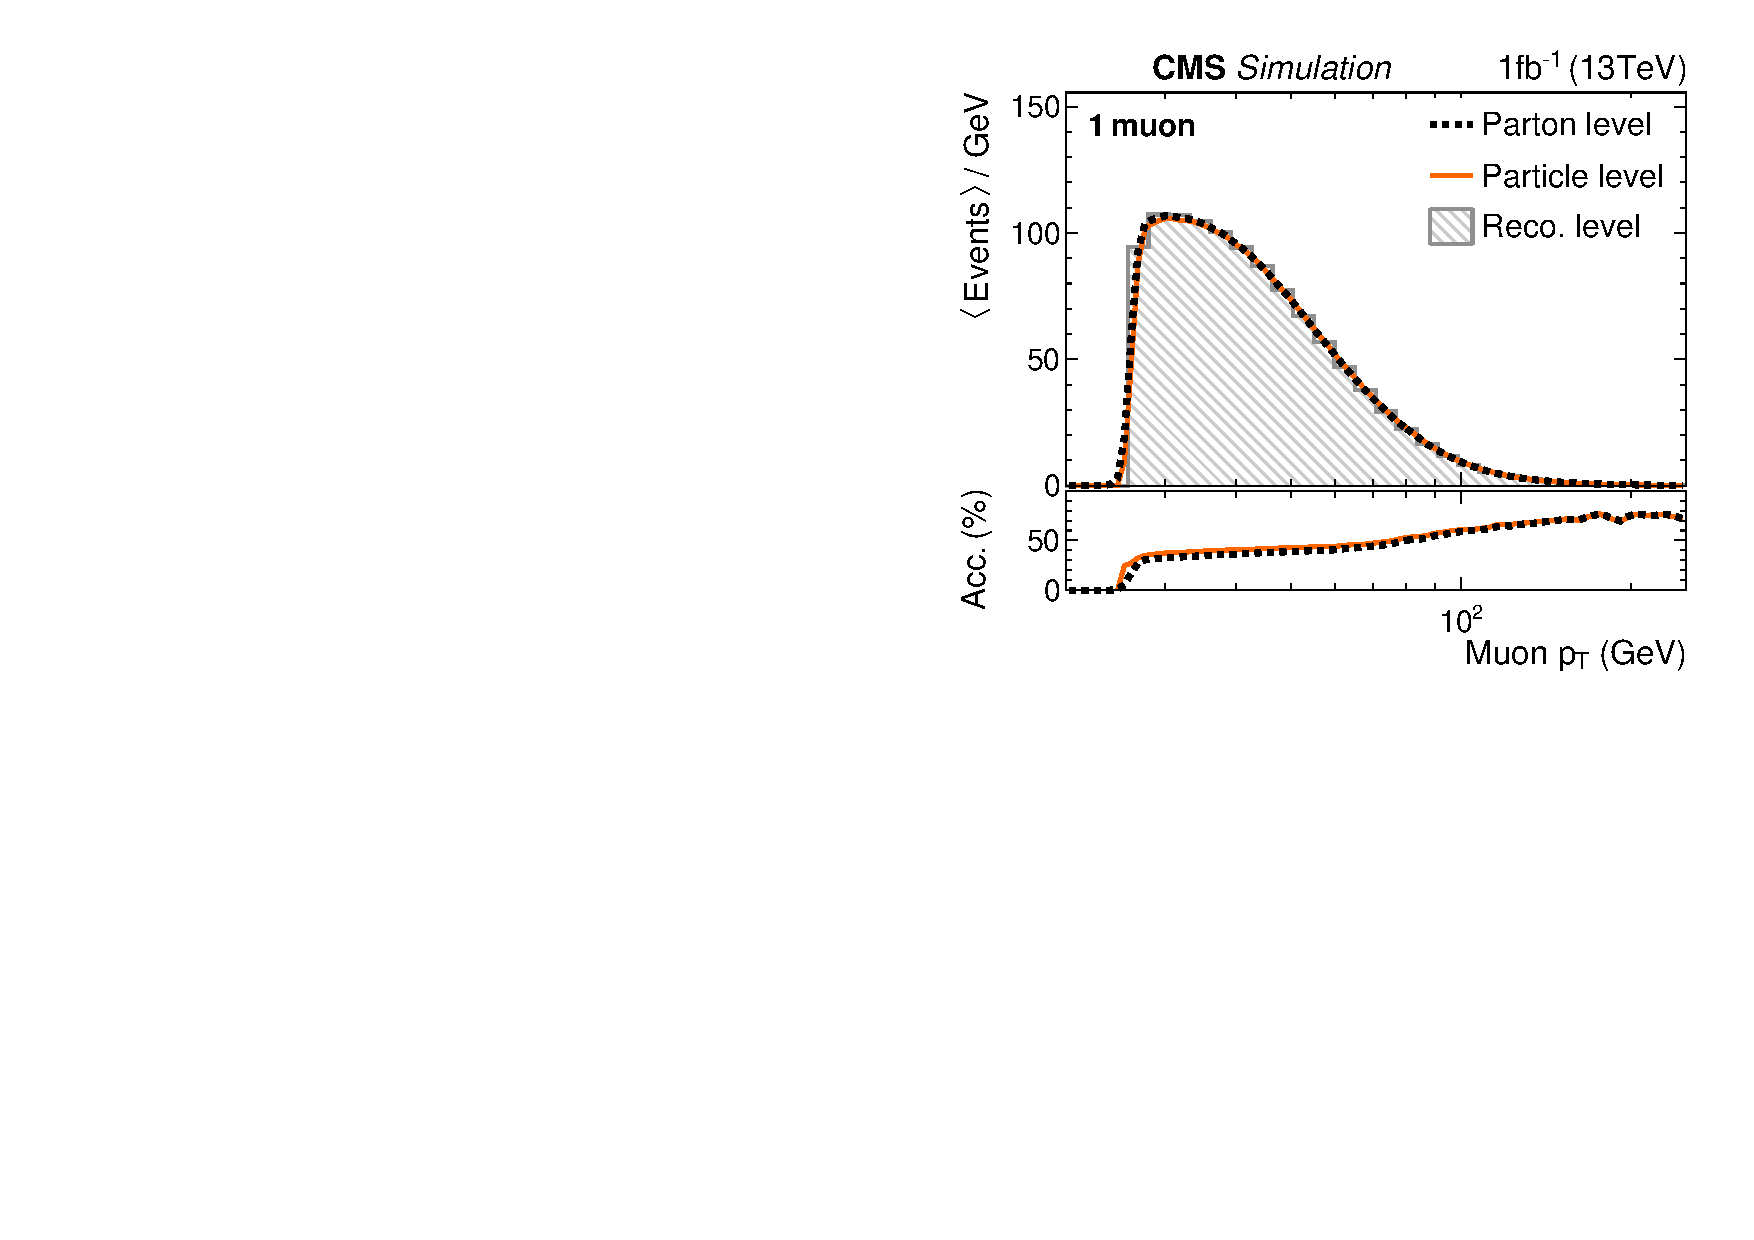
\includegraphics[width=0.48\textwidth]{figures/prospects/fiducial/muon_particle_logpt.pdf}}\hspace{0.03\textwidth}
\subfloat[\label{fig:prospects-particle-level-muoneta}]{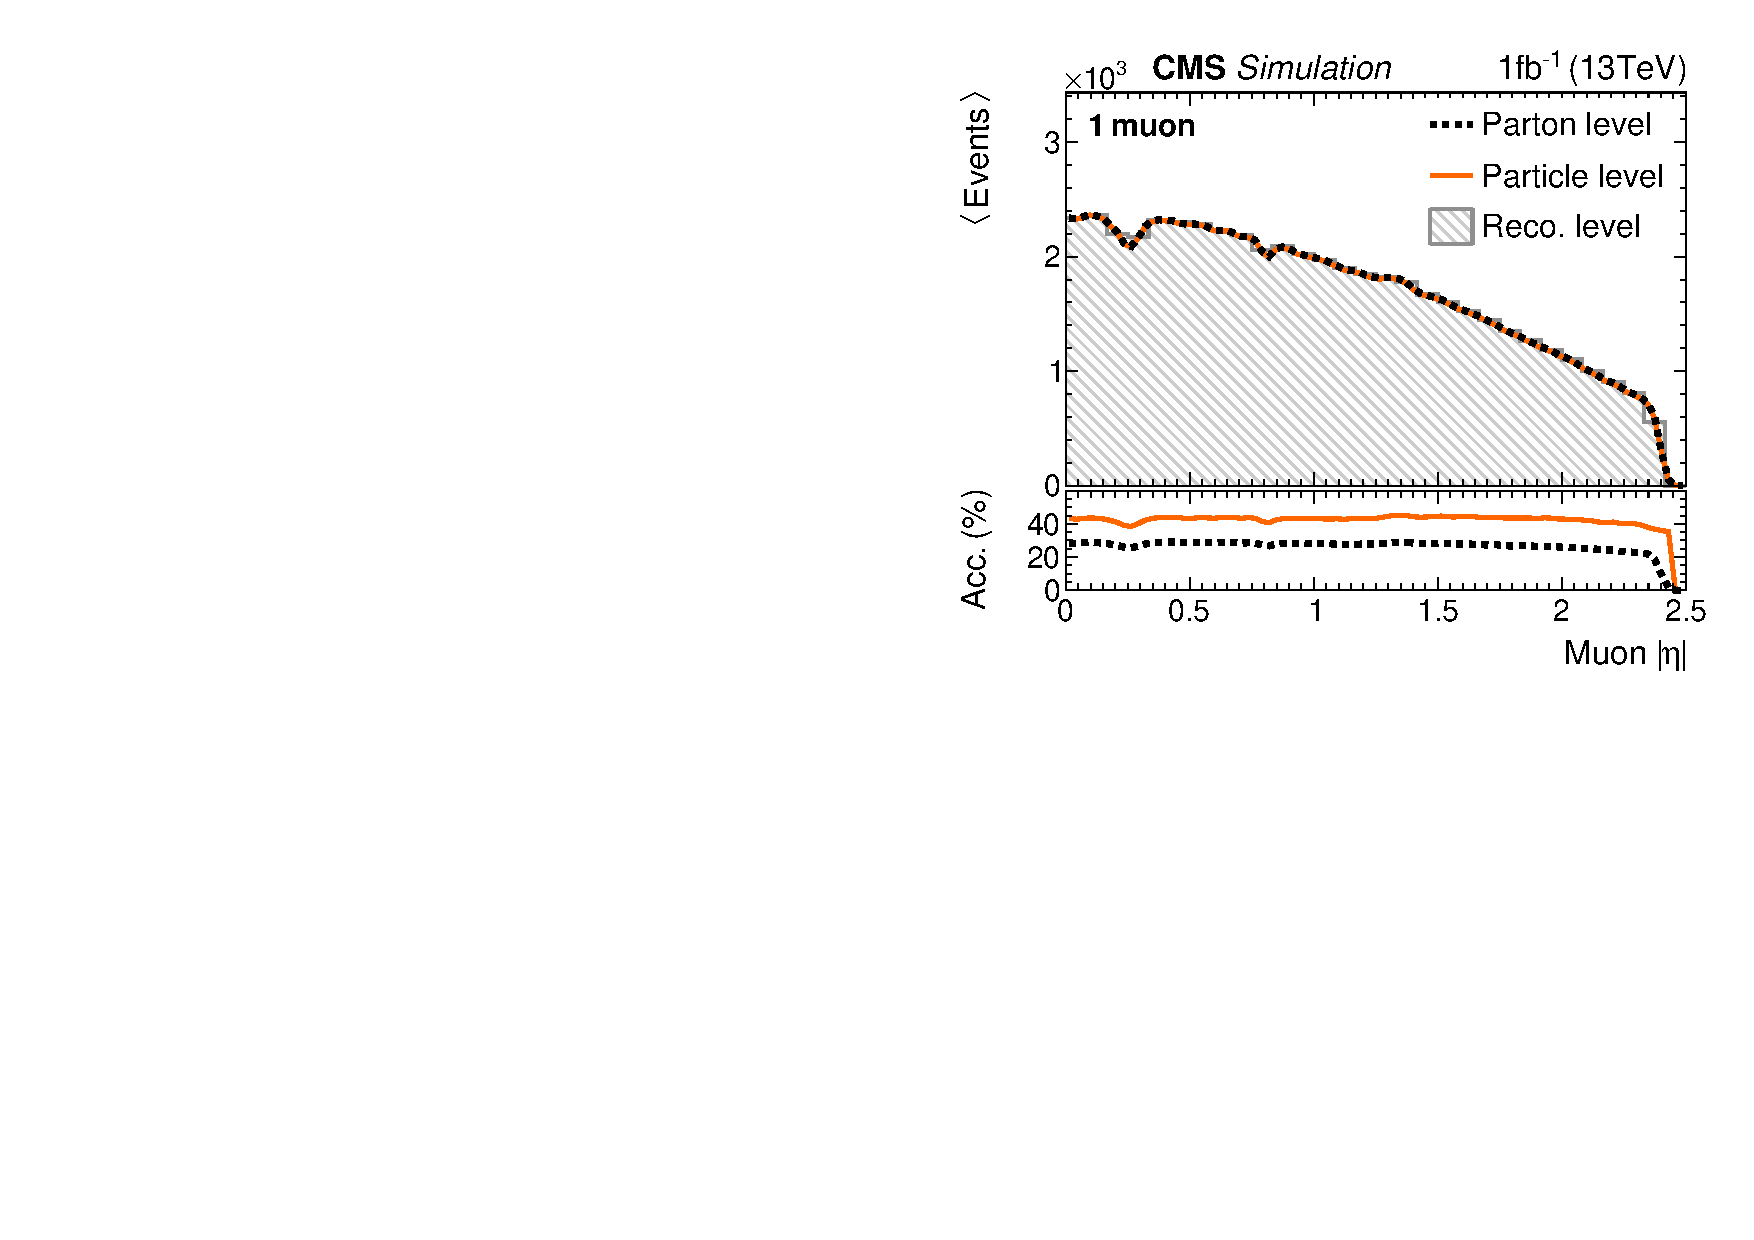
\includegraphics[width=0.48\textwidth]{figures/prospects/fiducial/muon_particle_abseta.pdf}}\\
\subfloat[\label{fig:prospects-particle-level-njet}]{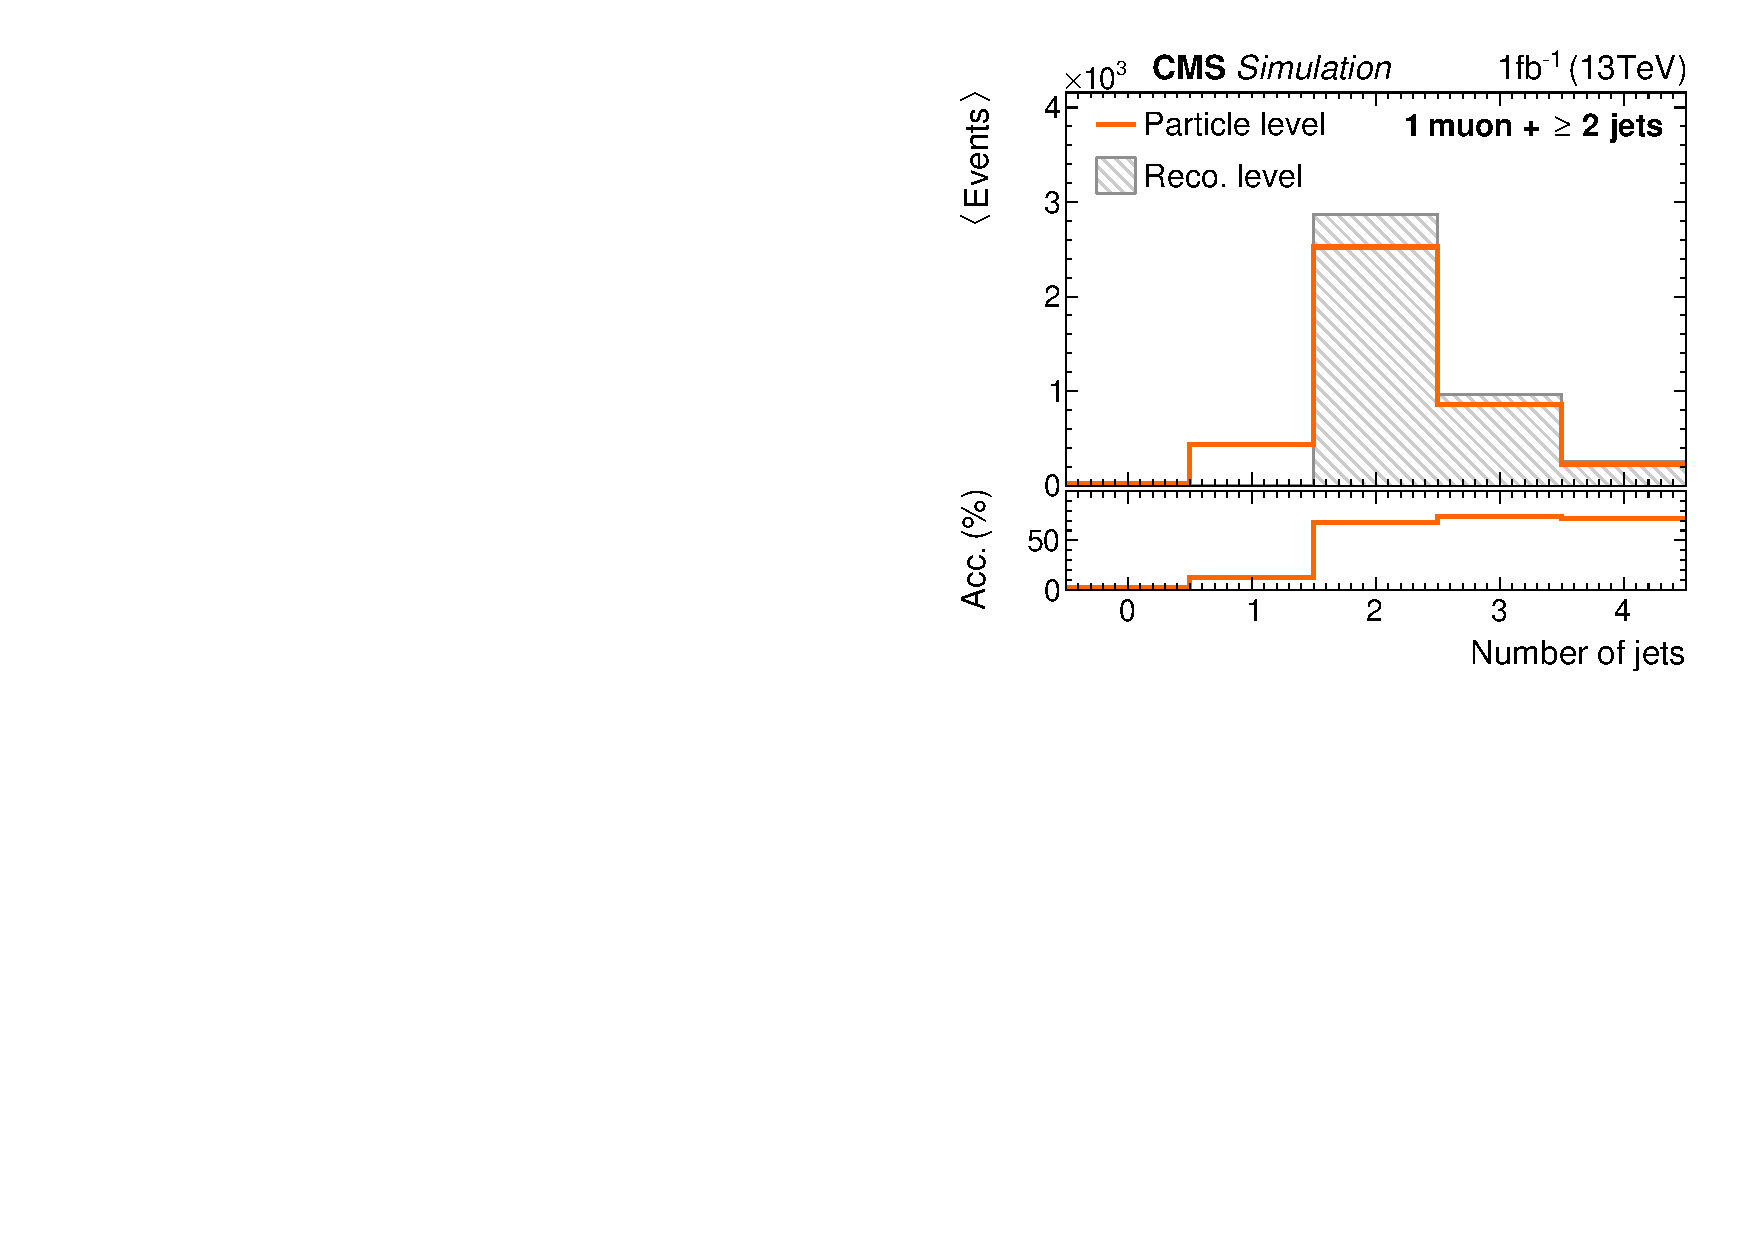
\includegraphics[width=0.48\textwidth]{figures/prospects/fiducial/njet_particle.pdf}}\hspace{0.03\textwidth}
\subfloat[\label{fig:prospects-particle-level-nbjet}]{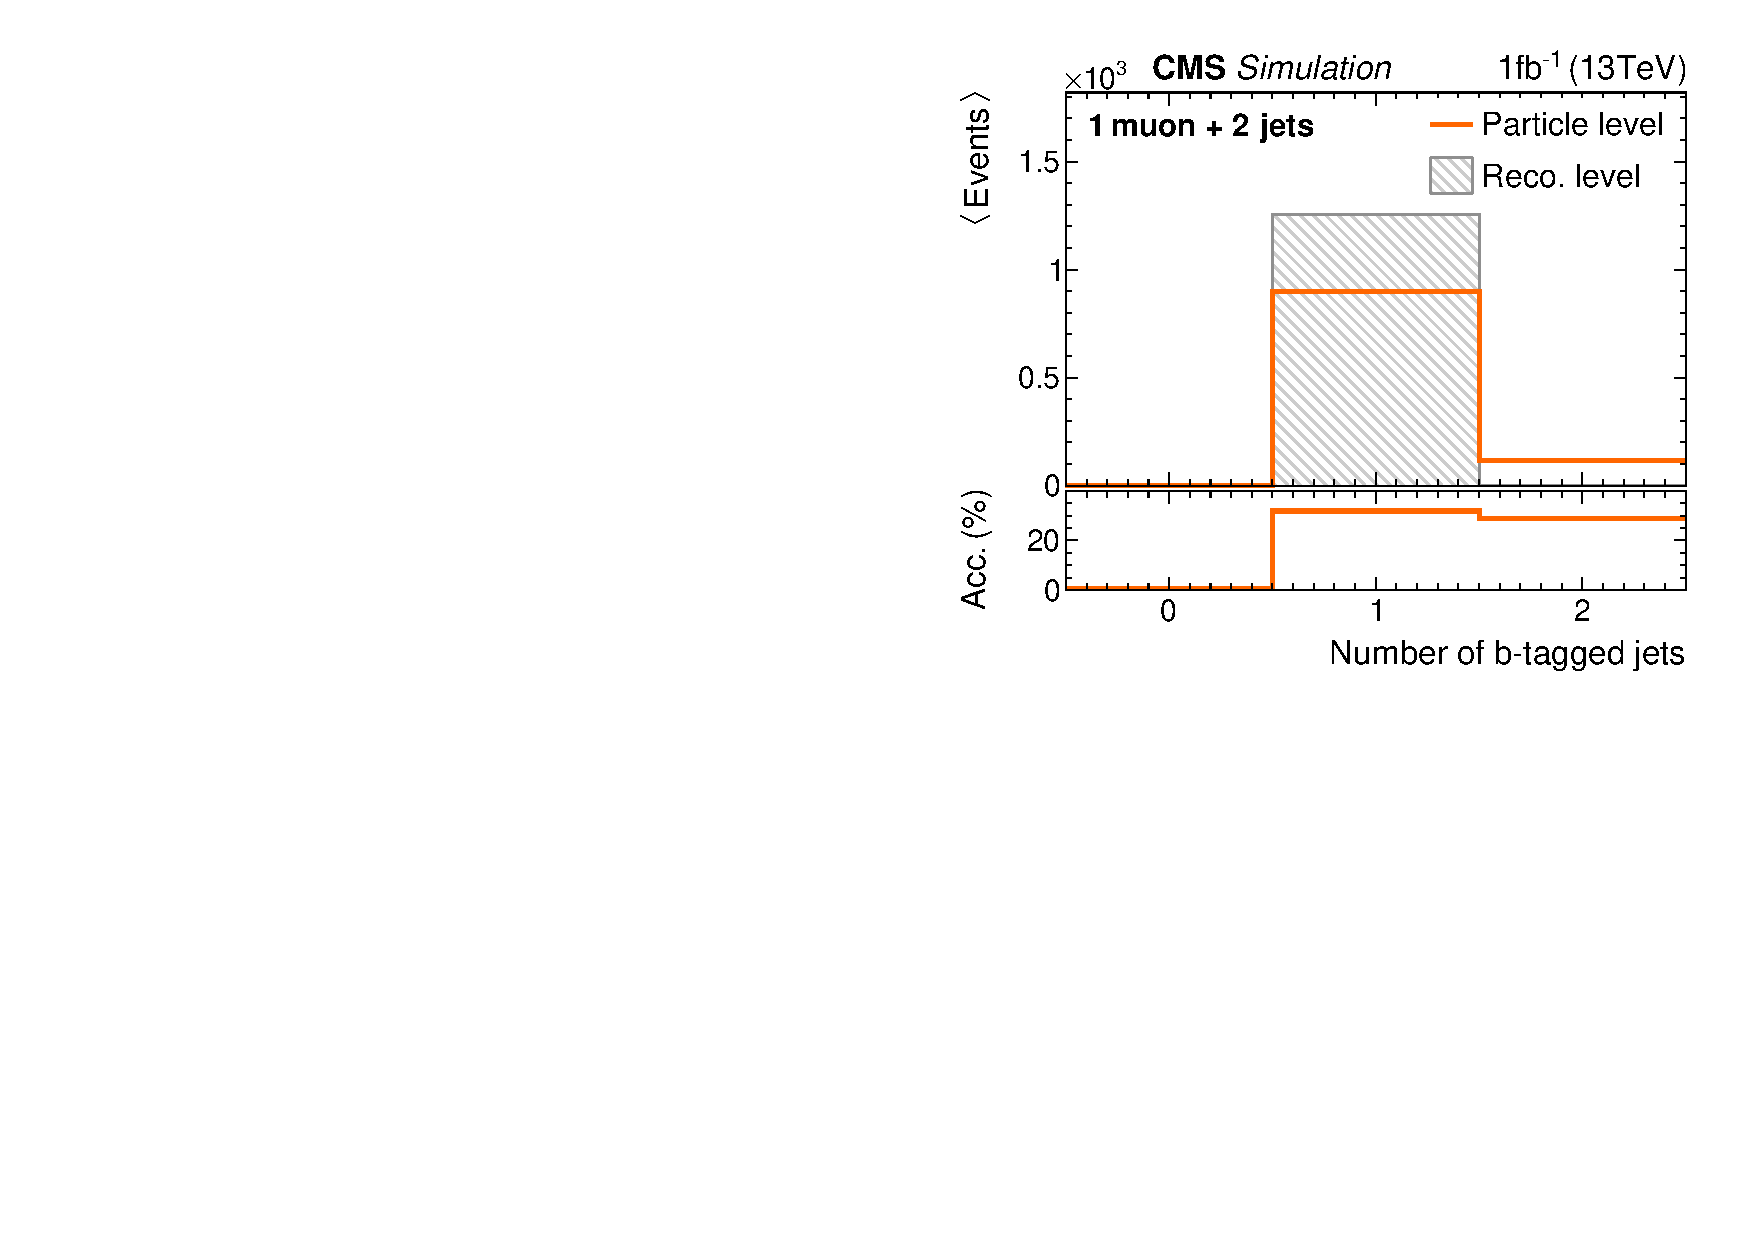
\includegraphics[width=0.48\textwidth]{figures/prospects/fiducial/nbjet_particle.pdf}}\\
\subfloat[\label{fig:prospects-particle-level-ljetpt}]{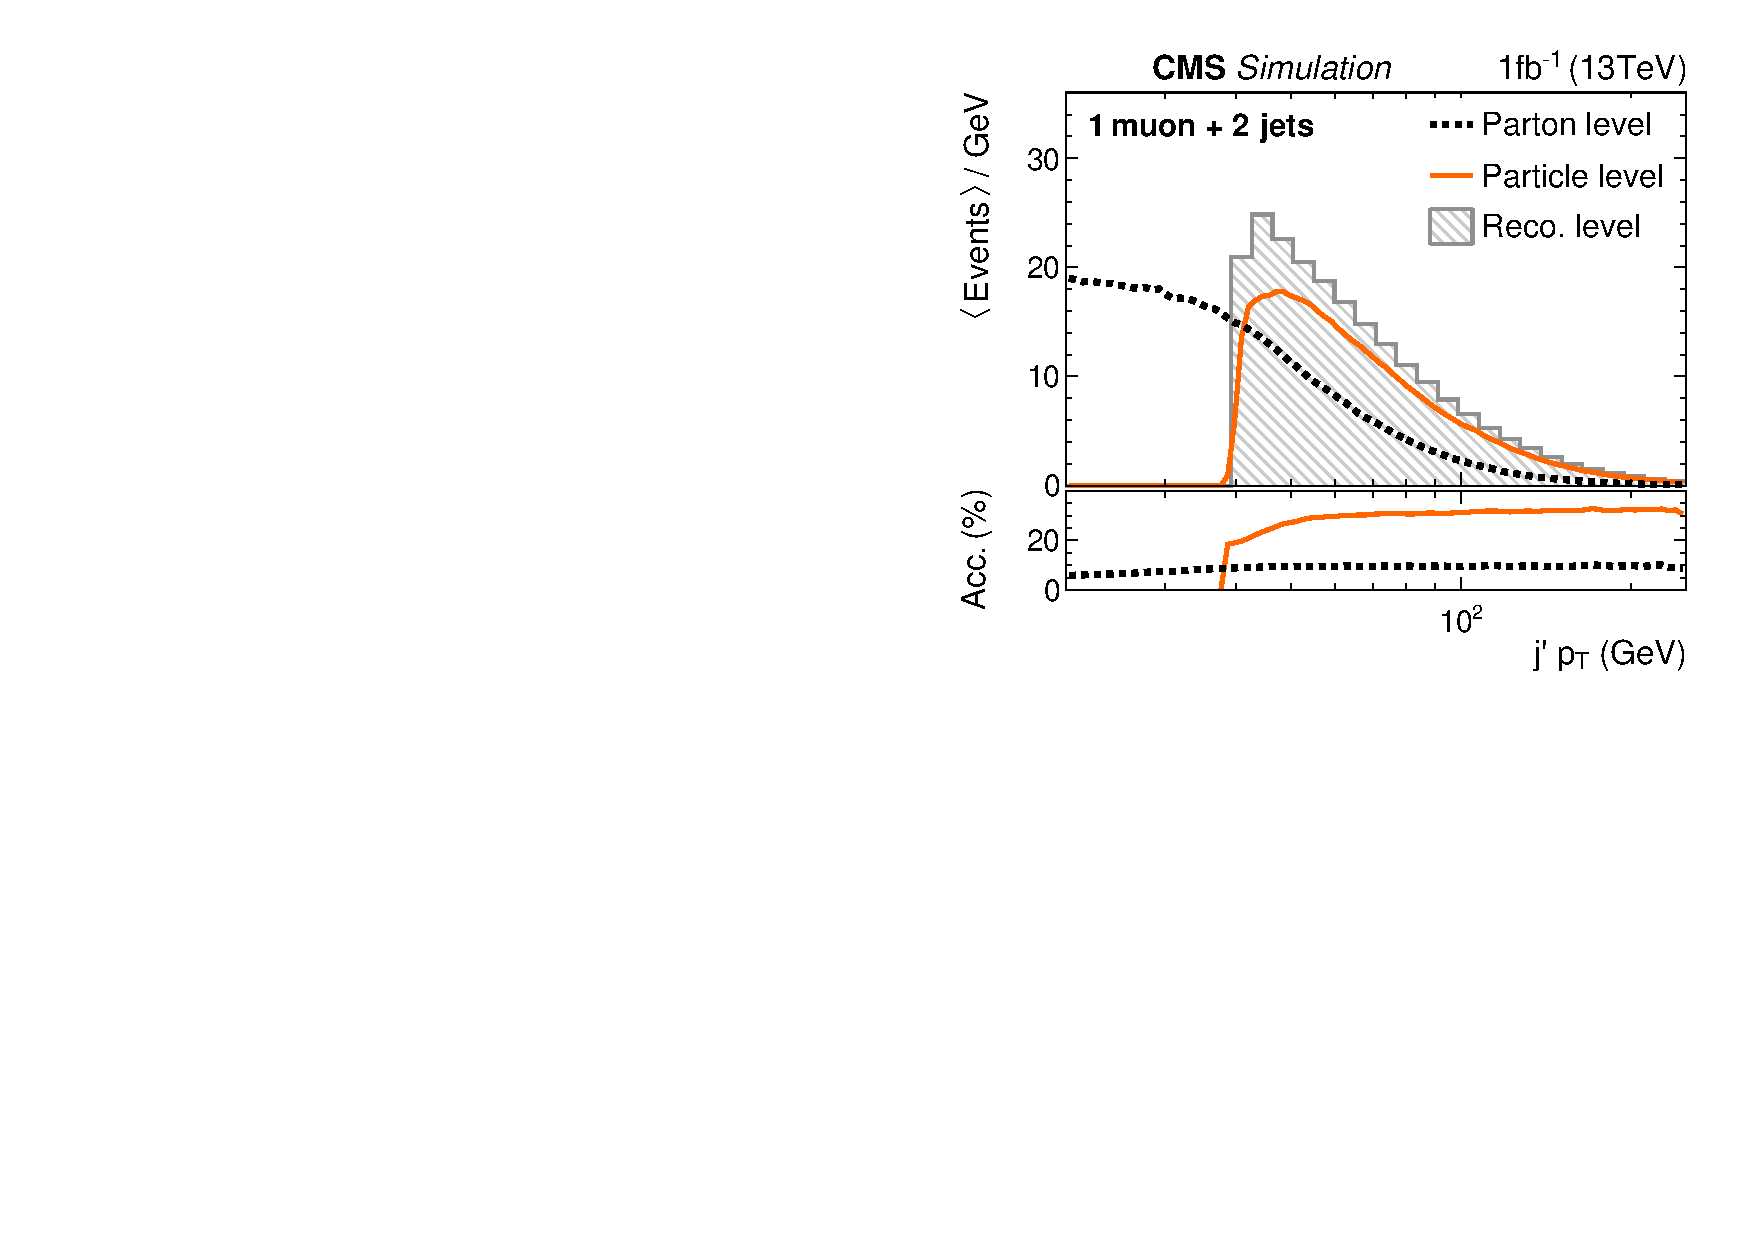
\includegraphics[width=0.48\textwidth]{figures/prospects/fiducial/ljet_particle_logpt.pdf}}\hspace{0.03\textwidth}
\subfloat[\label{fig:prospects-particle-level-ljeteta}]{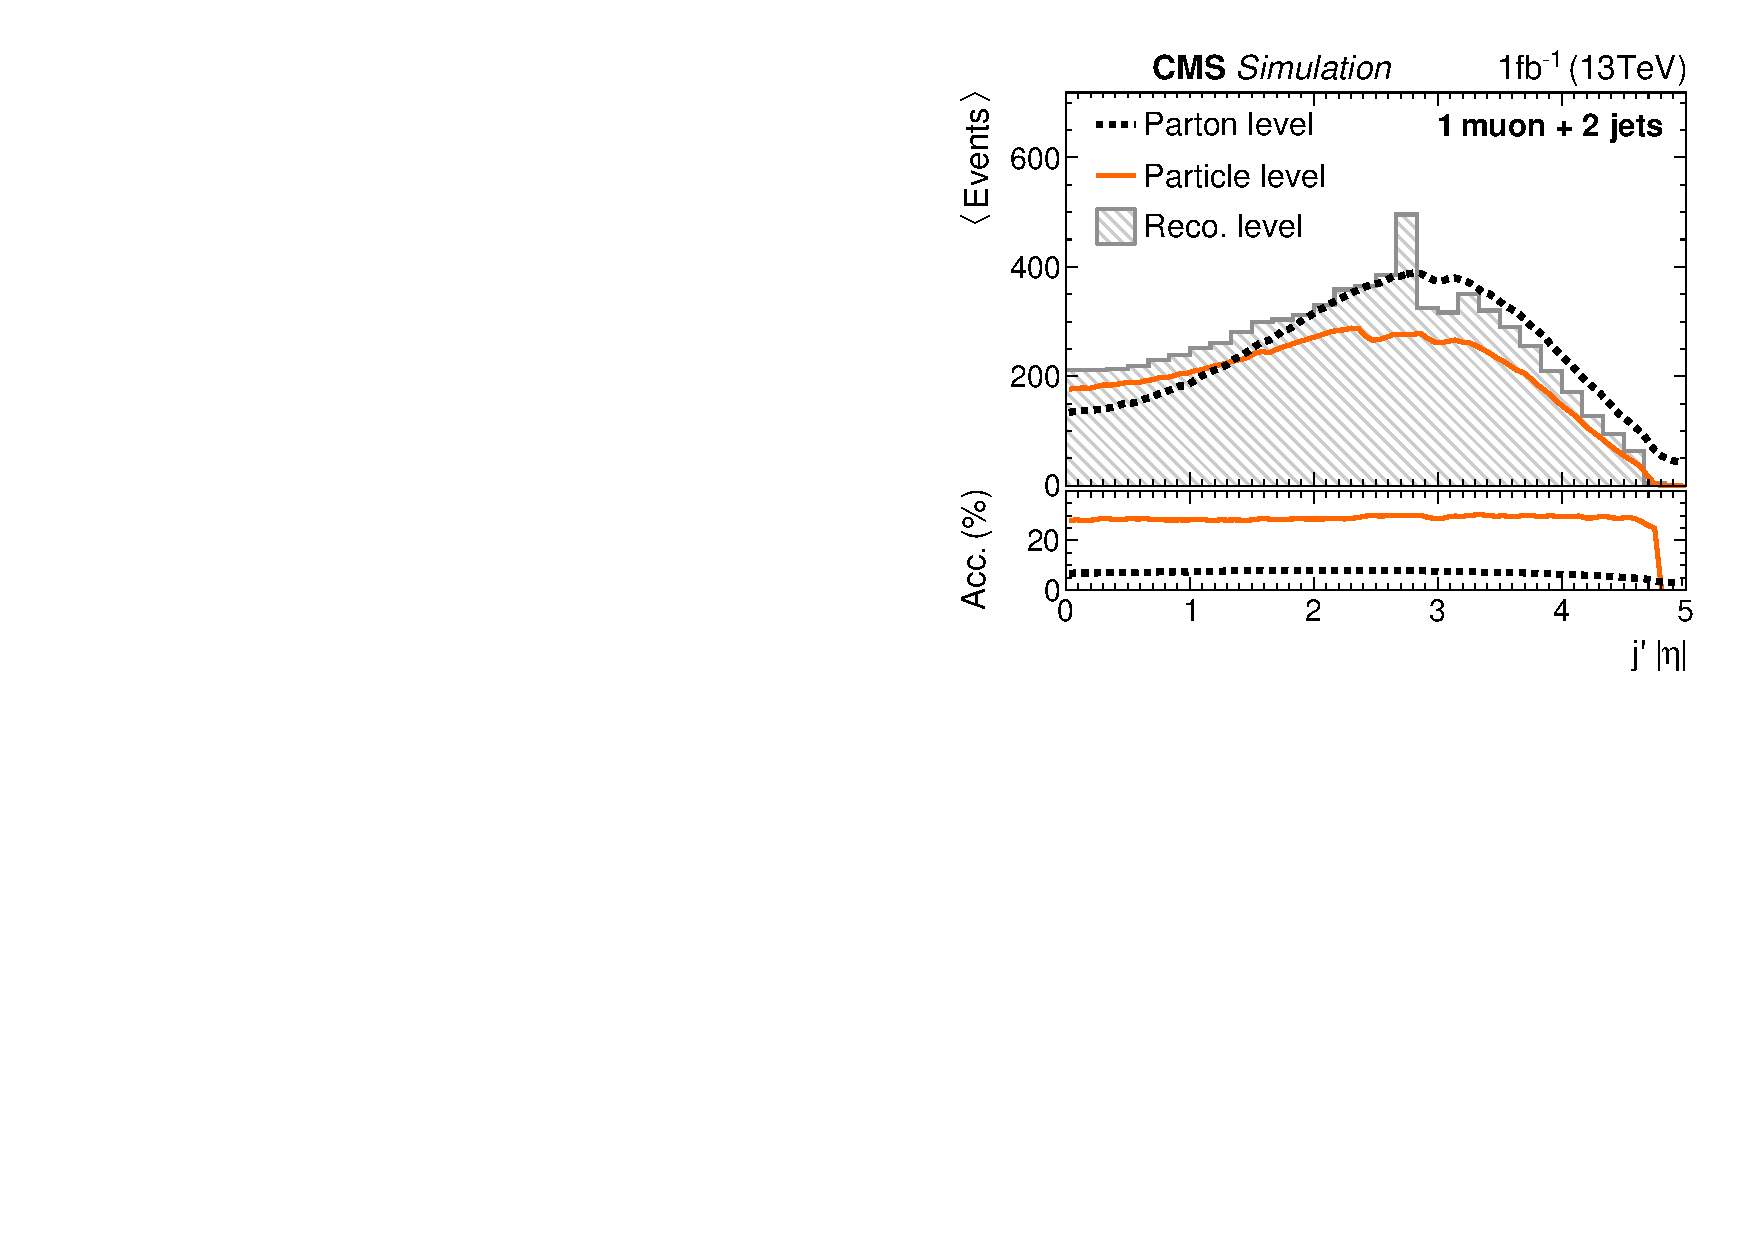
\includegraphics[width=0.48\textwidth]{figures/prospects/fiducial/ljet_particle_eta.pdf}}
}

\myfigure[phtb]{\label{fig:prospects-particle-top}Comparison of event selection at reconstruction and particle level.}{
\subfloat[]{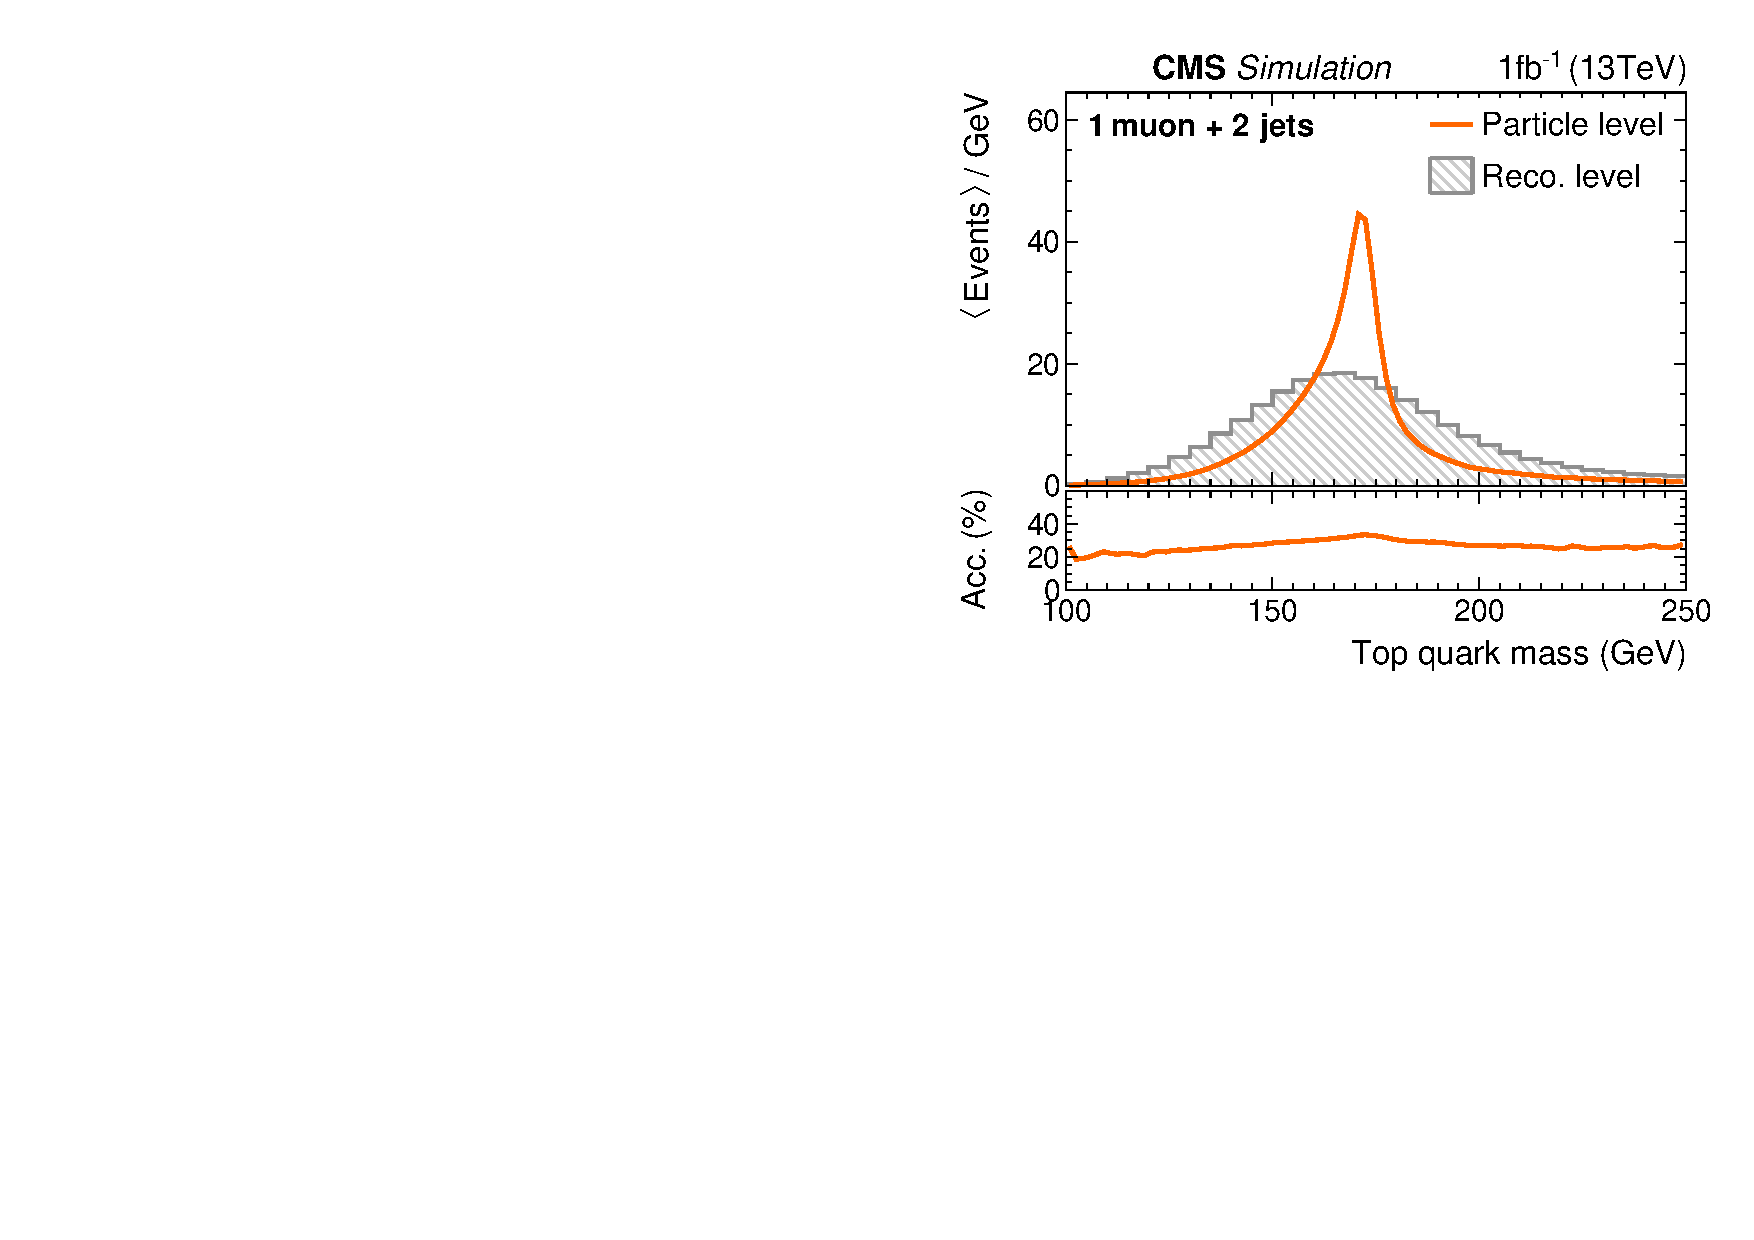
\includegraphics[width=0.48\textwidth]{figures/prospects/fiducial/top_particle_mass.pdf}}\hspace{0.03\textwidth}
\subfloat[]{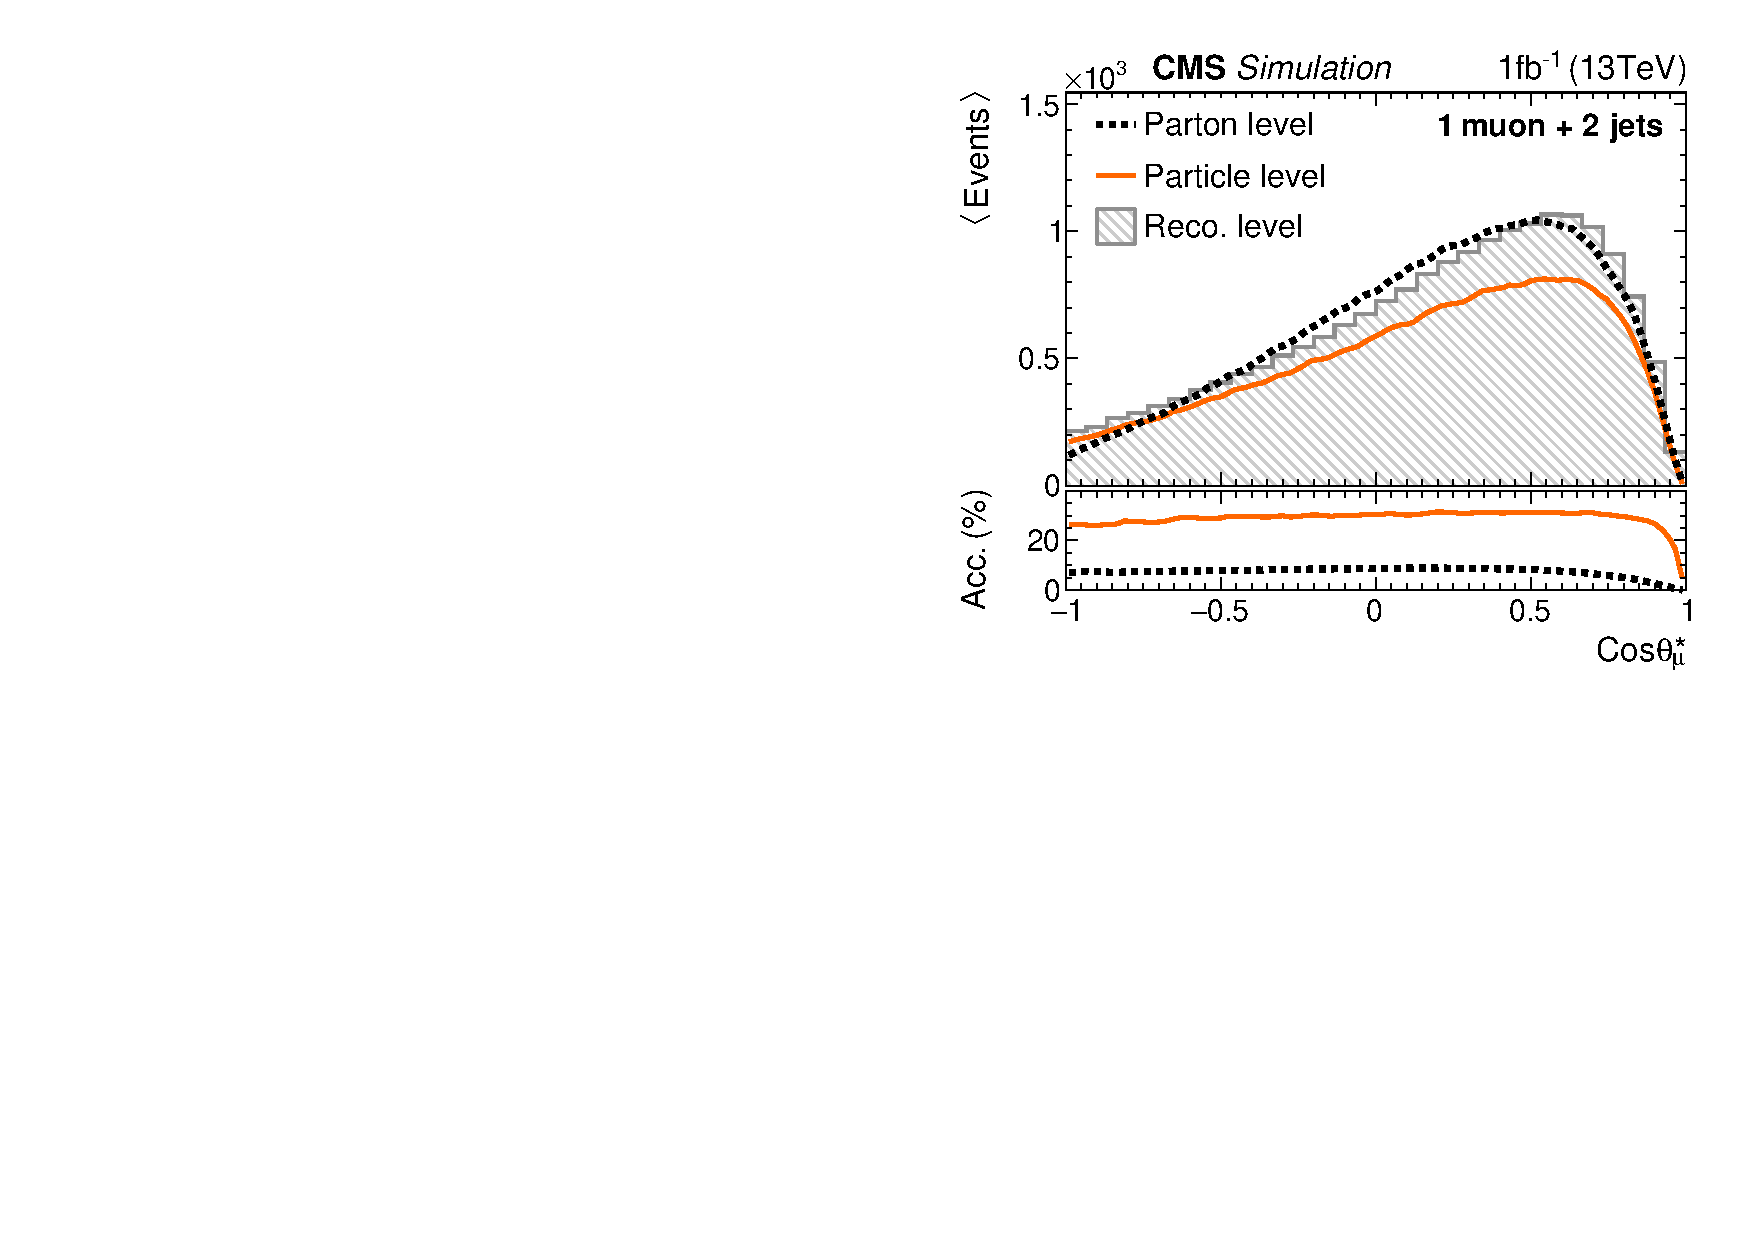
\includegraphics[width=0.48\textwidth]{figures/prospects/fiducial/cosTheta_particle.pdf}}
}

%############################################## 
\section{Validation}
%############################################## 

\myfigure[p]{\label{fig:pospects-validation}Validation in 2j1t control region (defined by $\bdttch<0$) of distributions in the (left column)~electron and (right column)~muon channel  .}{
\subfloat[]{\adjincludegraphics[height=4.8cm,trim={0 0 {0.16\width} 0},clip]{figures/prospects/plots/2j1t/electron_2j1t_top_pt_CR_nol.pdf}}
\subfloat[]{\adjincludegraphics[height=4.8cm,trim={0 0 {0.\width} 0},clip]{figures/prospects/plots/2j1t/muon_2j1t_top_pt_CR.pdf}}\\
\subfloat[]{\adjincludegraphics[height=4.8cm,trim={0 0 {0.16\width} 0},clip]{figures/prospects/plots/2j1t/electron_2j1t_top_absy_CR_nol.pdf}}
\subfloat[]{\adjincludegraphics[height=4.8cm,trim={0 0 {0.\width} 0},clip]{figures/prospects/plots/2j1t/muon_2j1t_top_absy_CR.pdf}}\\
\subfloat[]{\adjincludegraphics[height=4.8cm,trim={0 0 {0.16\width} 0},clip]{figures/prospects/plots/2j1t/electron_2j1t_cosTheta_tPL_CR_nol.pdf}}
\subfloat[]{\adjincludegraphics[height=4.8cm,trim={0 0 {0.\width} 0},clip]{figures/prospects/plots/2j1t/muon_2j1t_cosTheta_tPL_CR.pdf}}
}



%##############################################
\subsection{Excepted results on pseudo-data}
%##############################################